\chapter{Measurement of Weak Lensing and the Cosmic Microwave Background}
\section{Weak Lensing}
In general, contemporary weak lensing surveys measure the light emitted from galaxies in two components: galaxy position and galaxy shear. In the following sections, the theoretical base for cosmological weak lensing surveys are described. However, before discussing the two relevant observables, one needs to formalize the concept of weak lensing.
\begin{figure}[ht]
	\centering
	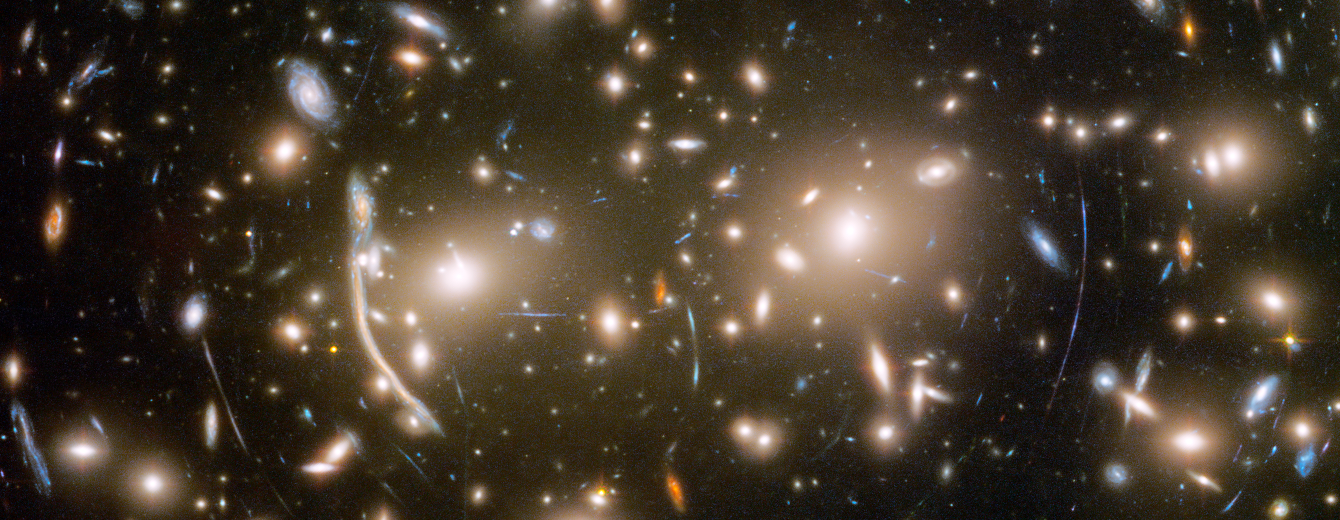
\includegraphics[width=\textwidth]{plots/hubble_weak_lensing.png}
	\caption{Image of weak lensing taken by the Hubble Space Telescope~\cite{hubble_lensing}.}
	\label{fig:weak_lensing}
\end{figure}
\subsection{The Linear Matter Power Spectrum}
As was seen before, deviations from the FLRW metric are represented by the scalar fields $\Phi$ and $\Psi$. In the absence of anisotropic stress, $\Phi=-\Psi$, which is a good approximation for the late universe\footnote{One can use codes such as \textsc{CAMB}~\cite{antony_lewis_camb_nodate} to do computations including anisotropy.}. 

Throughout time in the universe, there are three distinct epochs~\cite{scott_dodelson_modern_2021}:
\begin{itemize}
	\item The super-horizon region. At early times, the horizon $\eta$ is small, and the Fourier modes $k$ for all except the smallest scales are beyond the horizon ($k\eta\ll1$).
	\item The horizon-crossing region. At intermediate times with rapid inflation, the horizon grows quickly. Fourier modes which were previously beyond the horizon cross into the horizon ($k\eta\approx1$).
	\item The sub-horizon region. At late times, all Fourier modes except the larges scales remain within the horizon ($k\eta\gg1$).
\end{itemize}
Additionally, the formation of matter inhomogeneity comes from gravitational instability. Primordial curvature perturbations sourced initial inhomogeneity, which evolved under gravitational forces to become the galaxies and clusters seen today.

This description provides a blueprint for writing the matter power spectrum. There is the primordial curvature perturbation $\mathcal{R}$ which source the initial matter inhomogeneity that formed late-time large-scale structure. Thus, it can be written as
\begin{equation}
	\mathcal{R} = \frac{5}{3}\Phi_{\text{large-scale}}(k,a_{\text{late}})\,.
\end{equation} 
Additionally, there is a transfer function which describes the transition from radiation to matter domination, defined as
\begin{equation}
	T(k) = \frac{\Phi(k,a_{\text{late}})}{\Phi_{\text{large-scale}(k,a_{\text{late}})}}\,.
\end{equation}
And there is a growth factor, defined as the linear growth of matter density contrast during matter domination, defined as
\begin{equation}
	D_+(a) = a \frac{\Phi(k,a)}{\Phi(k,a_{\text{late}})}\,.
\end{equation}
Thus the gravitational potential at all times can be written as
\begin{equation}
	\Phi(k,a) = \frac{3}{5a}\mathcal{R}(k)T(k,a)D_+(a)\,.
\end{equation}
This together with the Poisson equation for the matter density contrast field gives the equation
\begin{equation}
	\delta_m(k) = \frac{2k^2a}{3\Omega_mH_0^2}\Phi(k,a)\,,
\end{equation}
\begin{equation}
	\delta_m(k) = \frac{2}{5}\frac{k^2}{\Omega_mH_0^2}\mathcal{R}(k)T(k,a)D_+(a)\,.
\end{equation}
The power spectrum of an observable is defined as the two-point correlation function of the observable in Fourier space.
\begin{equation}
	P_\mathcal{O}(k) = \langle \mathcal{O}(k)\mathcal{O}(k) \rangle
\end{equation}
Thus, the linear matter power spectrum\footnote{Linear comes from the fact that only linear terms in the equations of motion for the matter density are kept} is given by
\begin{equation}
	\begin{split}
		P_m^{L}(k,a) = \frac{8\pi^2}{25 \Omega_m^2 H_0^4} A_s D_+^2(a)T^2(k)\frac{k^{n_s}}{k_p^{(n_s-1)}}\,.
	\end{split}
\label{eq:power_spectrum}
\end{equation}

\subsection{Galaxy Density}
In practice, it is impossible to directly measure the power spectrum; dark matter prohibits direct measurement. Instead, one must determine observables which trace the matter distribution in the universe. The most natural option is to observe the galaxy distribution, where galaxies also form due to gravitational interaction with dark matter. Galaxy density is a biased tracer of the full matter density, so the galaxy and matter power spectra are related by a linear bias factor.
\begin{equation}
	\begin{split}
		\delta_g(k) &= b_1 \delta_m(k) \\
		P_g(k,a) &= (b_1)^2P_m^L(k,a)
	\end{split}
\end{equation}
Realistically, galaxy surveys do not have access to exact redshifts for each observed galaxy. Rather, an image is taken of the sky in multiple color bands, from which the redshift is determined. This measurement is called photometric redshift. To account for this, one can attempt to redefine the galaxy power spectrum. First, define the distribution of distances as
\begin{equation}
	W(\chi) = \frac{1}{N_g}\frac{dN_g}{d\chi}\,.
\end{equation}
The procedure for determining this distribution will be discussed in section~\ref{sec:dz}. This allows one to simply write the projected density contrast as
\begin{equation}
	\Delta_g = \int\limits_0^\infty W(\chi)\delta_g(x,\tau)d\chi\,.
\end{equation}
To complete this discussion, some approximations must be made. The first is that only consider small scales for which $\sin(\theta)\sim \theta \sim 1/l$ are considered, where $l$ is the Fourier conjugate of $\theta$. The second is the limber approximation, which states that, as long as the galaxy power spectrum $P_g$ slowly varies over the region $\Delta k \sim 1/l\chi$, $P_g$ can be approximated as a constant. These approximations greatly simplify the integrals required when computing the power spectrum of the Fourier transformed $\Delta_g$. This power spectrum is called the angular power spectrum. Considering the approximations above and computing the Fourier transform, one finds an angular power spectrum of
\begin{equation}
 	C_g(l) =\int \frac{1}{\chi^2}W^2(\chi)P_g(k=(l+1/2)/\chi,\eta) d\chi\,.
\end{equation} 
\subsection{Galaxy Shear}
Photons move on null geodesics, thus $d\chi = -d\eta$, where $\eta$ is the conformal time and $\chi$ is the conformal distance. This tells us that, through some changes of variables, $dx^i/d\chi = -\hat{p}^i$ (for photons and other massless particles). Thus, under lensing, the difference between the observed and true positions within the source plane is given by
\begin{equation}
	\chi\mathbf{\theta}^i = x_\perp^i = -\int\limits_0^\chi \hat{p}^i_\perp(\chi'') d\chi''\,.
\end{equation}
The goal is to write this as a function of the potential only. Thus, one must compute $d\hat{p}^i/dt$.
\begin{equation}\label{eq:dp-hat-dt}
	\begin{split}
		\frac{d\hat{p}^i}{dt} %=& \frac{d}{dt}\frac{1}{p}p^i \\
		=& \frac{1}{p^2}(\dot{p}^i p - \dot{p}p^i)
	\end{split}
\end{equation}
By computing $\dot p^i$, one can find $\dot p$ as well:
\begin{equation}
	\begin{split}
		\frac{dp^i}{d\lambda} %=& \frac{d}{d\lambda}\left(aP^i(1+\Phi)\right) \\
		=& P^i\frac{d}{d\lambda}(a(1+\Phi)+(1+\Phi)a\frac{d}{d\lambda}P^i\,.
	\end{split}
\end{equation}
Also, $d/d\lambda = P^\mu \partial_\mu$, so the first term becomes
\begin{equation}
	\begin{split}
		P^i\frac{d}{d\lambda}(a(1+\Phi)) %&= P^iP^\mu \partial_\mu(a(1+\Phi)) \\
		%&= P^iP^0(\dot a + a\dot\Phi + \dot a \Phi) + a P^iP^j \partial_j\Phi \\
		&= a P^i (P^0(H+\dot\Phi +H\Phi) + P^j\partial_j\Phi)\,. \\
	\end{split}
\end{equation}
The second term is evaluated by using the geodesic equation up to first order in the perturbations $\Phi$ and $\Psi$.
\begin{equation}
	\begin{split}
		\frac{d}{d\lambda}P^i &= -\Gamma^i_{\mu\nu}P^\mu P^\nu \\
		%&= -(P^0)^2\frac{1}{a^2}\partial^i\Psi - 2\delta^{i}_{j}(H+\dot\Phi)P^0P^j + 2P^iP^j\partial_j\Phi - P^jP_j\partial^i\Phi \\
		%&= -E(1-\Psi)\left( \frac{E}{a^2} \partial^i\Psi + \frac{1}{a}2p^i(1-\Phi)(H+\dot\Phi) - \frac{2}{a^2E}p^ip^j\partial_j\Phi + \frac{p^2}{a^2E} \partial^i\Phi \right) \\
		&= -E\left( \frac{E}{a^2} \partial^i\Psi + \frac{1}{a}2p^i(1-\Phi-\Psi)(H+\dot\Phi) - \frac{2}{a^2E}p^ip^j\partial_j\Phi + \frac{p^2}{a^2E} \partial^i\Phi \right)\,.
	\end{split}
\end{equation}
Plugging everything back in, and only keeping terms to linear order, one gets
\begin{equation}
	\begin{split}
		%=& aP^i(H+\dot\Phi+H\Phi) + aP^iP^j\partial_j\Phi \\
		%& - \frac{E}{a}\partial^i\Psi - 2p^i(H+\dot\Phi) + \frac{2}{aE}p^ip^j \partial_j\Phi - \frac{p^2}{aE}\partial^i\Phi \\
		\frac{dp^i}{dt} %=& p^i(1-\Phi)(H+\dot\Phi+H\Phi) + (1-\Phi)^2p^ip^j\partial_j\Phi \\
		%& - \frac{E}{a^2}\partial^i\Psi -\frac{2p^i}{a}(H+\dot\Phi) + \frac{2}{a^2E}p^ip^j \partial_j\Phi - \frac{p^2}{a^2E}\partial^i\Phi \\
		%=& p^i(H+\dot\Phi) + \frac{p^ip^j}{aE}\partial_j\Phi \\
		%& - \frac{E}{a}\partial^i\Psi -2p^i(H+\dot\Phi) + \frac{2}{aE}p^ip^j \partial_j\Phi - \frac{p^2}{aE}\partial^i\Phi \\
		=& -p^i(H+\dot\Phi)- \frac{1}{aE}\left(p^ip^j\partial_j\Phi - p^2\partial^i\Phi\right) -\frac{E}{a}\partial^i\Psi\,.
	\end{split}
\end{equation}
The time derivative of the modulus of the momentum, $p$, is then given by
\begin{equation}
	\begin{split}
		\frac{dp}{dt} =& \frac{d}{dt}\sqrt{\delta_{ij}p^ip^j} = \frac{1}{p}\delta_{ij}\dot p^i p^j \\
		%=& -p(H+\dot\Phi) - \frac{p}{aE}(p^i\partial_i\Phi - pp^i\partial^i\Phi) - p^i\frac{E}{ap}\partial^i\Psi \\
		=& -p(H+\dot\Phi) - \hat{p}_i\frac{E}{a}\partial^i\Psi\,.
	\end{split}
\end{equation}
Now, putting everything together, plugging these results into equation~\ref{eq:dp-hat-dt} gives
\begin{equation}
	\begin{split}
		\frac{d\hat{p}^i}{dt} %=& -\hat{p}^i(H+\dot\Phi)- \frac{1}{aEp}\left(p^ip^j\partial_j\Phi - p\partial^i\Phi\right) -\frac{E}{ap}\partial^i\Psi + \hat{p}^i\left( (H+\dot\Phi) + \hat{p}_i\frac{E}{ap^2}\partial^i\Psi \right) \\
		=&  \frac{E}{ap}\left( \frac{p^2}{E^2}\partial_j\Phi - \partial_j\Psi \right)(\delta^{ij}-\hat{p}^i\hat{p}^j)\,.
	\end{split}
\end{equation} 
Going back to the photon scenario, where $E=p$, this simplifies to
\begin{equation}
	\frac{d\hat{p}^i}{dt} = \frac{1}{a}\left( \partial_j\Phi - \partial_j\Psi \right)(\delta^{ij}-\hat{p}^i\hat{p}^j)\,.
\end{equation}
Interestingly, $\delta^{ij}-\hat p^i \hat p^j$, is the projection operator of the $j$-th direction onto the $i$-th. So, if one orients the axes so that the photon approximately travels along the $j$-th direction, one can sum of $i$ and $k$ so that the orthogonal components of the momentum are evaluated by
\begin{equation}
	\frac{d\hat{p}^i_\perp}{d\chi} = - a \frac{d\hat{p}^i_\perp}{dt} = -\partial_i(\Phi-\Psi)\,.
\end{equation}
In the absence of anisotropic stress, $\Phi=-\Psi$ and 
\begin{equation}
	\frac{d\hat{p}^i_\perp}{d\chi} -2\partial_i\Phi\,.
\end{equation}
Integrating this equation gives
\begin{equation}
	\hat p_\perp (\chi'') = -2\int\limits_0^{\chi''}\partial_i\Phi(\chi') d\chi' + C_i\,,
\end{equation}
where the constant $C_i$ comes from integrating a derivative, where it is only defined up to a constant. Plugging this back in one finds
\begin{equation}
	\mathbf{\theta}^i = \frac{2}{\chi}\int\limits_0^\chi \int\limits_0^{\chi''}\partial_i\Phi(\chi') d\chi' d\chi'' - C_i\,.
\end{equation}
In the absence of lensing, this should reduce to $\mathbf{\theta}^i = \theta_0$, the true source position. Hence $C^i=\theta^i_0$ and the total deflection angle is given by
\begin{equation}
	\begin{split}
		\Delta\theta^i =& \frac{2}{\chi}\int\limits_0^\chi \int\limits_0^{\chi''}\partial_i\Phi(\chi') d\chi' d\chi''\\
		=& \frac{2}{\chi}\int\limits_0^\chi \partial_i\Phi(\chi') (\chi-\chi') d\chi'\,.
	\end{split}
\end{equation}
Finally, since $x^i=\chi\theta^i$, $\partial_i = \partial_{\theta^i}/\chi$. Introduce the \textit{lensing potential} defined by
\begin{equation}
	\begin{split}
		\Delta\theta^i =& \frac{\partial}{\partial \theta^i}\psi_L(\theta) \\
		\psi_L(\theta) =& 2\int\limits_0^\chi \frac{1}{\chi'}\Phi(\chi') \left(1-\frac{\chi'}{\chi}\right) d\chi'\,.
	\end{split}
\end{equation}
This result is great, but it's not very experimentally illuminating. Similar to the galaxy versus matter power spectrum, the inability to directly measure the dark matter distribution means the potential $\Phi$ cannot be determined. Again, an attempt to relate the lensing potential to some property of galaxies can give a measurable quantity. However, it can be seen that lensing distorts the shape of the galaxies (figure~\ref{fig:weak_lensing}), where it is assumed all galaxies are elliptical. Define the galaxy shape tensor by
\begin{equation}
	q_{ij} \equiv \frac{1}{F}\int I\theta^i\theta^j d\theta^i d\theta^j\,.
\end{equation}
This integral is symmetric under $i \leftrightarrow j$. Writing this as a matrix gives
\begin{equation}
	q_{ij} = \frac{1}{2} \text{tr}(q) \left( 
	\begin{array}{cc}
	1+\epsilon_1 & \epsilon_2 \\
	\epsilon_2 & 1-\epsilon_1
	\end{array}
	\right)\,.
\end{equation}
Shape distortion occurs when the deflection angle is not constant across a galaxy. One can look at the transformation tensor as
\begin{equation}
	A_{ij} \equiv \frac{\partial \theta^i_S}{\partial\theta^j} = \left( 
	\begin{array}{cc}
	1+\kappa - \gamma_+ & -\gamma_\times \\
	-\gamma_\times & 1+\kappa+\gamma_+
	\end{array}
	\right) = \delta_{ij}+\psi_{ij}\,.
\end{equation}
Within this tensor, the $\gamma_+$ and $\gamma_-$ terms represent shear and $\kappa$ represents magnification and changes in galaxy light flux. The $E$-mode is given by
\begin{equation}
	E(l) = \left( \frac{l^il^j}{l^2} - \frac{1}{2}\delta^{ij} \right)(-\psi^{ij}(l))\,.
\end{equation}
Which relates to the shear components by
\begin{equation}
	\left(
	\begin{array}{c}
	\gamma_+ \\
	\gamma_\times
	\end{array}
	\right)
	=
	\left(
	\begin{array}{c}
	\cos(2\alpha_l) \\
	\sin(2\alpha_l)
	\end{array}
	\right)
	E(l)\,.
\end{equation}
This connects the observable shear to the theoretical lensing potential.
\subsection{Weak Lensing Correlation Functions}
In the previous two sections, two observables directly connected to cosmological theories were defined. Observing the galaxies can determine $\Omega_b$, $A_s$, $n_s$ and $H_0$. Observing shear can determine $\Omega_m$ (the details of how to determine these parameters will be discussed in chapter 3). Together, these two can fully determine the values of the 5 $\Lambda$CDM parameters. These two quantities, however, are not measurable. Using these two quantities, however, one can construct three different two-point correlation functions which are measurable.

The first correlation function is the autocorrelation of galaxy density, called galaxy clustering and denoted $w_\theta$. Given a density in a particular angular position, the correlation function can be interpreted as the likelihood of observing a similar density at another close position. The galaxy clustering correlation function is given by
\begin{equation}
	w_g(\theta) = \mathcal{F}(C_g(l)) = \frac{1}{2\pi}\int\limits_0^\infty l C_g(l) J_0(l\theta)dl\,,
\end{equation}
where $J_0$ is the zeroth Bessel function and $\mathcal{F}$ denotes the Fourier transform.

Next is the shear autocorrelation. In this case, there are two components of shear: the tangential shear $\gamma_+$ and the cross shear $\gamma_\times$. The cross correlation $\langle \gamma_+ \gamma_\times \rangle$ vanishes, and the remaining combinations are
\begin{equation}
	\begin{split}
		\langle \gamma_+\gamma_+ \rangle \pm \langle \gamma_\times \gamma_\times \rangle = \xi_\pm
	\end{split}
\end{equation}
\begin{equation}
	\xi_{+,-} = \frac{1}{2\pi}\int\limits_0^\infty l C_{EE}(l) J_{0,4}(l\theta)C_{EE}(l)dl\,.
\end{equation}

The final observable is the cross correlation between galaxy density and tangential shear. First, the angular power spectrum $C_{gE}(l)$ is given by
\begin{equation}
	C_{gE}(l) = \frac{3}{2}\Omega_mH_0^2 \int\limits_0^\infty \frac{1}{\chi a(\chi)}W_g(\chi)P_g(k,\eta) d\chi\,,
\end{equation}
\begin{equation}
	\gamma = \langle \Delta_g\gamma_+\rangle = -\frac{1}{2\pi}\int\limits_0^\infty l J_2(l\theta)C_{gE}(l)dl\,.
\end{equation}
The correlation function $\langle \Delta_g\gamma_\times\rangle$ vanishes in an isotropic universe.

\subsection{Systematics}
Up to now, any systematics of the weak lensing observables have been ignored. There are two distinct types of systematics that will be discussed in this section: The ones which affect the calculation of the correlation functions, and the ones which affect the correlation functions after they have been computed. The latter type of parameters are usually referred to as `fast' parameters, and it will become clear why that is in the next chapter. Meanwhile, the ways the systematics are modelled is described here.
\subsubsection{Photometric Redshift Uncertainty}\label{sec:dz}
To compute the two-point correlation functions, one must determine the redshift distribution $W(\chi)$. This is a highly non-trivial task. To model the uncertainty in this distribution, one applies a constant shift to the redshift of observed galaxies.
\begin{equation}
	n_g(z) \mapsto n_g(z+\Delta z)
\end{equation}
The shift $\Delta z$ must be determined before one can compute the galaxy clustering and galaxy lensing correlation functions.
\subsubsection{Intrinsic Alignment of Galaxies}\label{sec:IA}
Galaxy shapes are not completely random. In the absence of lensing, there is still some non-zero correlation between the shapes. This is referred to as Intrinsic Alignment~\cite{troxel_intrinsic_2015,scott_dodelson_modern_2021}. There are two models of intrinsic alignment that will be considered in this thesis: the Tidal Alignment Tidal Torquing (TATT) model~\cite{krause_dark_2021,blazek_beyond_2019} and the Non-linear Alignment (NLA) model. The TATT depends on the tidal tensor $s_{ij}$, which contains the information about tidal forces due to non-uniform gravitational fields. Tidal forces are a source of intrinsic alignment and shear by stretching matter along the radial direction from the gravitational source. The model is given by
\begin{equation}
	\gamma_{ij}^I = \underbrace{C_1s_{ij}}_{\text{tidal alignment}}+
	\underbrace{b_{TA}C_1(\delta_m\times s_{ij})}_{\text{density weighting}}+
	\underbrace{C_2\left( s_i^ks_{kj}-\frac{1}{3}\delta_{ij}s^2 \right)}_{\text{tidal torquing}}\,,
\end{equation}
where the coefficients $C_a$ are given by
\begin{equation}
	\begin{split}
		C_1 =& -\frac{A_1\bar{C}\Omega_m}{aG(z)}\left(\frac{1+z}{1+z_0}\right)^{\eta_1} \\
		C_2 =& 5\frac{A_2\bar{C}\Omega_m}{(aG(z))^2}\left(\frac{1+z}{1+z_0}\right)^{\eta_2}\,.
	\end{split}
\end{equation}
The TATT model reduces to the NLA model when $A_2=0=b_{TA}$.
\subsubsection{Galaxy Bias}
The galaxy and matter density are related by a bias parameter $b$. However, a fiducial value can be chosen to relate the two:
\begin{equation}
	\delta_{g,\text{fid}} = b_{\text{fid}}\delta_m\,,
\end{equation}
then consider a multiplicative deviation:
\begin{equation}
	\delta_g = (b\cdot b_{\text{fid}})\delta_m = b\delta_{g,\text{fid}}\,,
\end{equation}
Thus, the parameter $b$ can be found to account for different galaxy biases. 

Galaxy bias is the first of many `fast' parameters. Since the bias is constant, it can be pulled out of the integral for the correlation functions, meaning it can be applied after the correlation function has been computed. The affected correlation functions are the galaxy clustering and galaxy-galaxy lensing.
\begin{equation}
	\begin{split}
		w^i(\theta) =& b_{(i)}^2w^i(\theta) \\
		\gamma^i_t(\theta) =& b_{(i)}\gamma_t^i(\theta)\,.
	\end{split}
\end{equation}
where $i$ denotes the redshift bin.
\subsubsection{Shear Calibration}
Observed shear is not completely caused by cosmological interactions. For example, a major source of additional shear comes from the observation lens itself, where the observed galaxy shape is given by the true galaxy shape convolved with the point spread function of the lens~\cite{hirata_shear_2003,gillis_effects_2019}. This is usually modelled as a multiplicative correction to the shear components.
\begin{equation}
	\begin{split}
		\xi^{ij}_{\pm} =& (1+m^i)(1+m^j) \xi^{ij}_{\pm} \\
		\gamma^{ij}_t =& (1+m^j) \gamma_t^{ij}\,,
	\end{split}
\end{equation}
where $i$ and $j$ denote the source and lens bin, respectively. The multiplicative shear calibration is also a fast parameter.
\subsubsection{Point Mass}
Currently, it is not possible to model the contribution of small scales to the tangential shear~\cite{maccrann_controlling_2020}. The tangential shear can be written in terms of the surface mass density $\Sigma$ tangential to the line of sight:
\begin{equation}
	\gamma_t(R/D_A) = \frac{\bar\Sigma(0,R) - \Sigma(R)}{\Sigma_\mathrm{crit}} = \frac{\Delta\Sigma(R)}{\Sigma_\mathrm{crit}}\,.
\end{equation}
The tangential shear can only be modelled down to scales of $r_\mathrm{min}$, which allows one to write the point mass contribution (named for the $R^{-2}$ dependence) as
\begin{equation}
	\Delta\Sigma(R) = \Delta\Sigma^{\mathrm{model}}(R) + \frac{B}{R^2}\,.
\end{equation}
\subsubsection{Lensing Magnification}
In weak lensing, the intrinsic shape of galaxies also gets magnified. This effect is introduced as a parameter $C_l^i$ and is fixed experimentally.

%Additionally, DES added a non-physical parameter called $X_{\text{lens}}$ to resolve an inconsistency between two lensing samples, RedMaGiC and MagLim. In this thesis, we only consider $X_{\text{\lens}}=1$

\section{CMB}
Although CMB data is not used sparsely in this thesis, it is worth discussing the measurements qualitatively~\cite{wayne_hu_animations_nodate,joshua_frieman_cmb_nodate,wayne_hu_thermal_nodate,hu_astro_nodate} The consensus among physicists and astronomers that the early universe was a hot, dense plasma. As such, the mean free path of photons was much shorter than it is today, and thus Compton scattering dominated photon dynamics in the early universe. As the universe cooled, atomic nuclei formed, and electrons began to bind to the nuclei in a process called recombination~\cite{scott_dodelson_modern_2021,wayne_hu_animations_nodate}. As the universe began to expand, the mean free path of photons increased and inter-atomic interactions decreased, meaning the amount of scattering was decreasing, until a point where photons are able to move freely through the universe.
\begin{equation}
	T = T_0(1-e^{-\tau_{\mathrm{rei}}})
\end{equation}
$\tau_{\mathrm{rei}}$ concludes the introduction of cosmological parameters. $\tau_{\mathrm{rei}}$ can only be determined from CMB and is usually fixed in weak lensing analysis.

The CMB is an almost-perfect black body, meaning the intensity of the light can be used to determine the temperature according to the black body equation where $I \propto T^4$. However, the imperfections source anisotropies in the temperature on the scale of $10^{-5}\,\mathrm{K}$. The temperature, along with the curl-free $E$-mode polarization, gives three possible two point correlation functions: $TT$, $TE$, and $EE$.
\subsection{\texorpdfstring{$TT$ Power Spectrum}{TT Power Spectrum}}
\begin{figure}
    \centering
    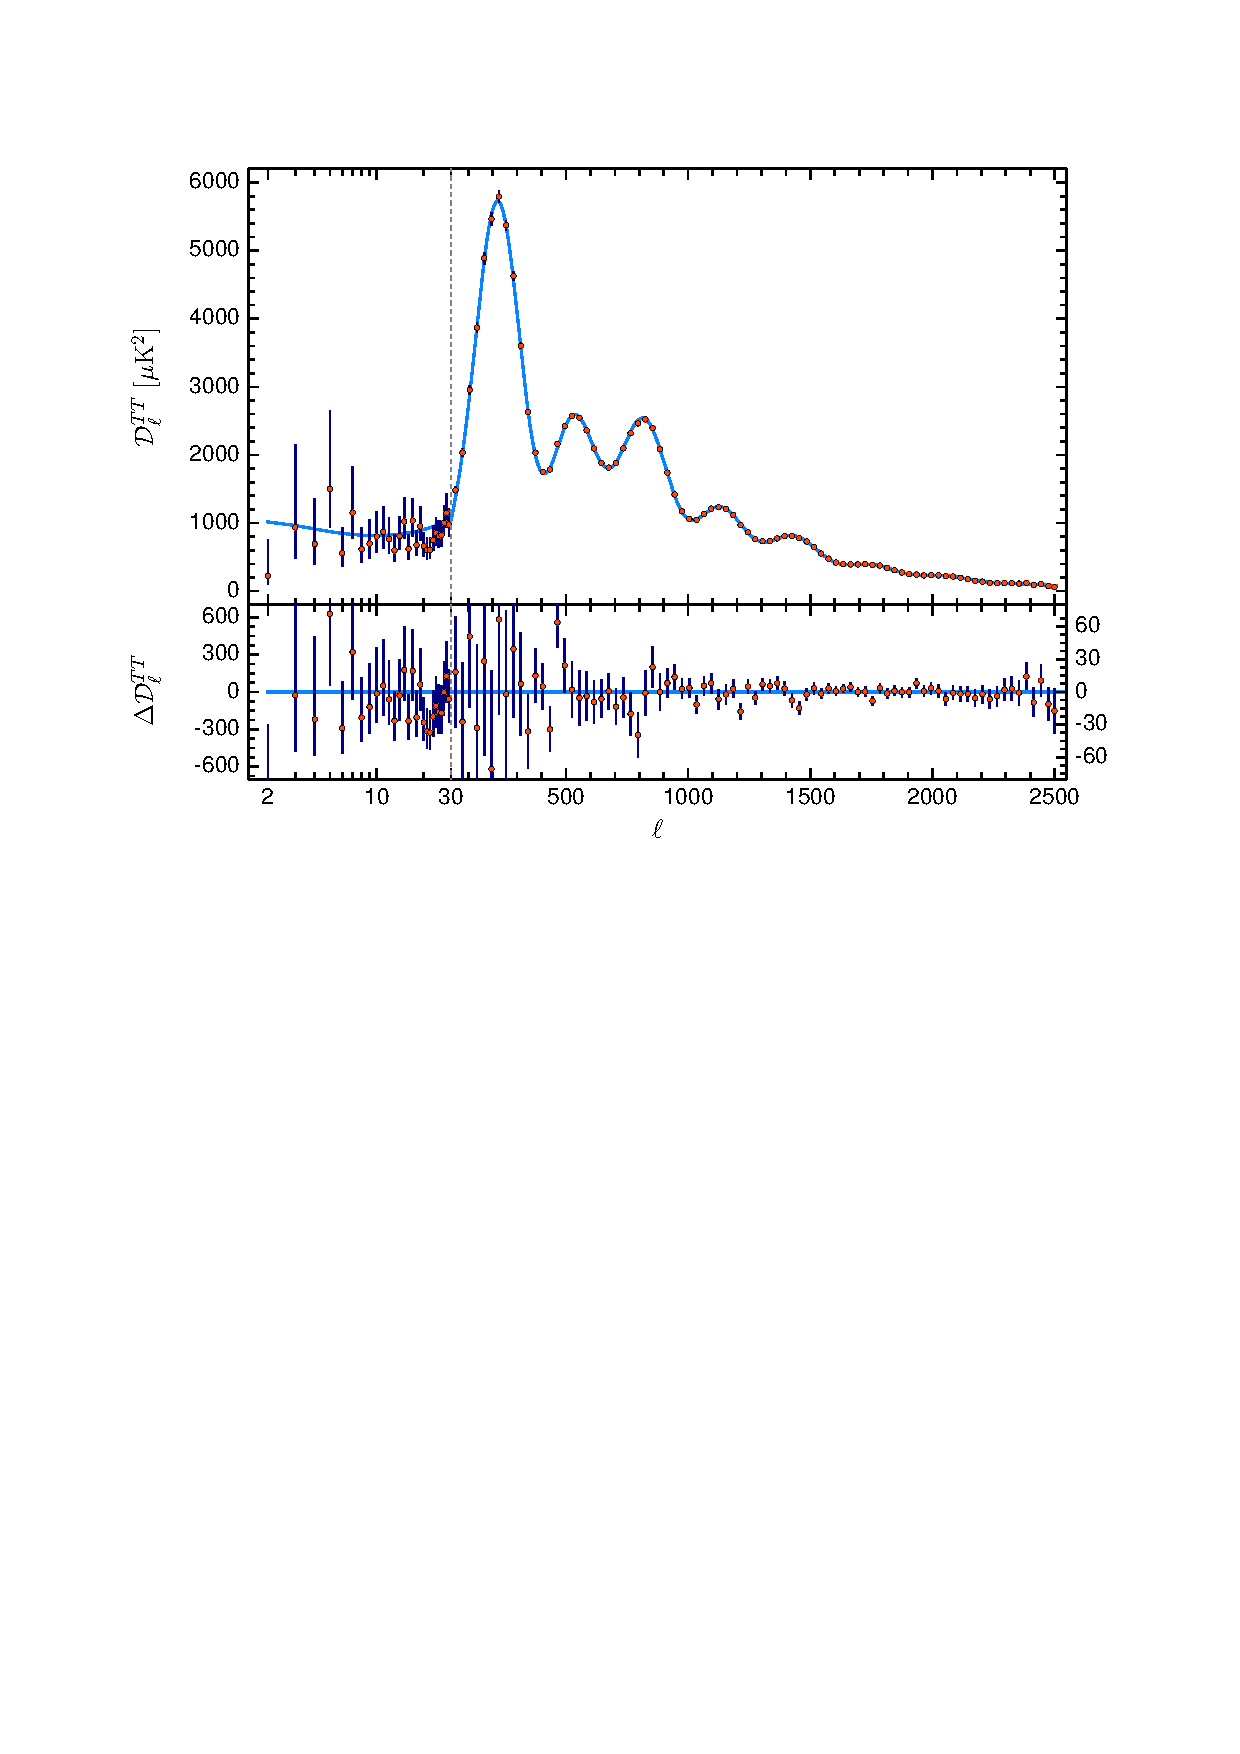
\includegraphics[width=0.9\textwidth]{plots/planck_tt.pdf}
    \caption{Planck $TT$ power spectrum~\cite{planck_collaboration_planck_2020}.}
    \label{fig:planck_tt}
\end{figure}
The $TT$ power spectrum measures the anisotropies of the temperature field. Thus, it is better to consider it as the deviation from the mean temperature. There are some prominent features of this spectrum worth discussing. The first is the oscillations, known as baryon acoustic oscillations. The second is the overall downward trend from large to small scales. This is generally due to diffusion of light through the early universe, and is given the name diffusion damping.

Now one can observe qualitatively how the cosmological parameters will affect the $TT$ power spectrum. First, consider $\Omega_b$, the baryon density. If the density is increased, there will be an increase in Compton scattering and a decrease in the mean free path of photons, meaning the large-scale anisotropy will be larger. Inversely, a reduction in the baryon density would decrease the large-scale anisotropy. This is typically observed as the height of the first peak in the $TT$ power spectrum. There will also be a small change in the peak position due to the change in the sound horizon. The height of the second peak, however, decreases. This is because an increase in baryon density causes an increase in the gravitational interactions between the baryons. This shifts down the oscillations in temperature contrast so that the acoustic oscillations occur around some negative value. Thus, in the $TT$ power spectrum, every other peak is enhanced.

Next is to consider a change is $\Omega_c$. The dominant effect from changing $\Omega_c$ comes from the integrated Sachs-Wolfe (ISW) effect, which is an additional gravitational redshift that occurs between the time of reionization and now. Since the evolution of dark matter structure is slow, increasing $\Omega_c$ reduces the ISW effect, thus reducing the anisotropy and causing an overall downward shift in the $TT$ power spectrum.

The remaining parameters are considered in unison: $\mathcal{A}_s$ and $\tau_{\mathrm{rei}}$. Naturally, $\tau_{\mathrm{rei}}$ will have an overall suppression effect. The amplitude is given by $\mathcal{A}_se^{-2\tau_{\mathrm{rei}}}$. Thus, the effect of $\mathcal{A}_s$ can look identical to changes in $\tau_\mathrm{rei}$. $n_s$, as before, defines the slope of the primordial power spectrum. Thus, changes to $n_s$ have a stronger effect on small scales than on large scales.

Finally, is a consideration of $H_0$, the most simple case. $H_0$ affects the expansion rate of the universe, thus a changing the value of $H_0$ will shift the position of the peaks in the power spectrum. Increases in $H_0$ will shift the peaks to smaller scales (found by propagating $H_0$ backward through time), and inversely, lowering $H_0$ will shift the peaks to larger scales. Additionally, the peaks at small scales will have a lower shift than the peaks at large scales. Hence, $H_0$ can also be determined by the distance between the peaks.

As a final remark, one can consider the curvature density $\Omega_k$. Changes in $\Omega_k$ affect the angular distance to recombination, resulting in an overall shift of the $TT$ power spectrum. Measurements strongly constrain this to $\Omega_k=0$, suggesting a flat universe.
\subsection{\texorpdfstring{$TE$ and $EE$ Power Spectra}{TE and EE Power Spectra}}
\begin{figure}
    \centering
    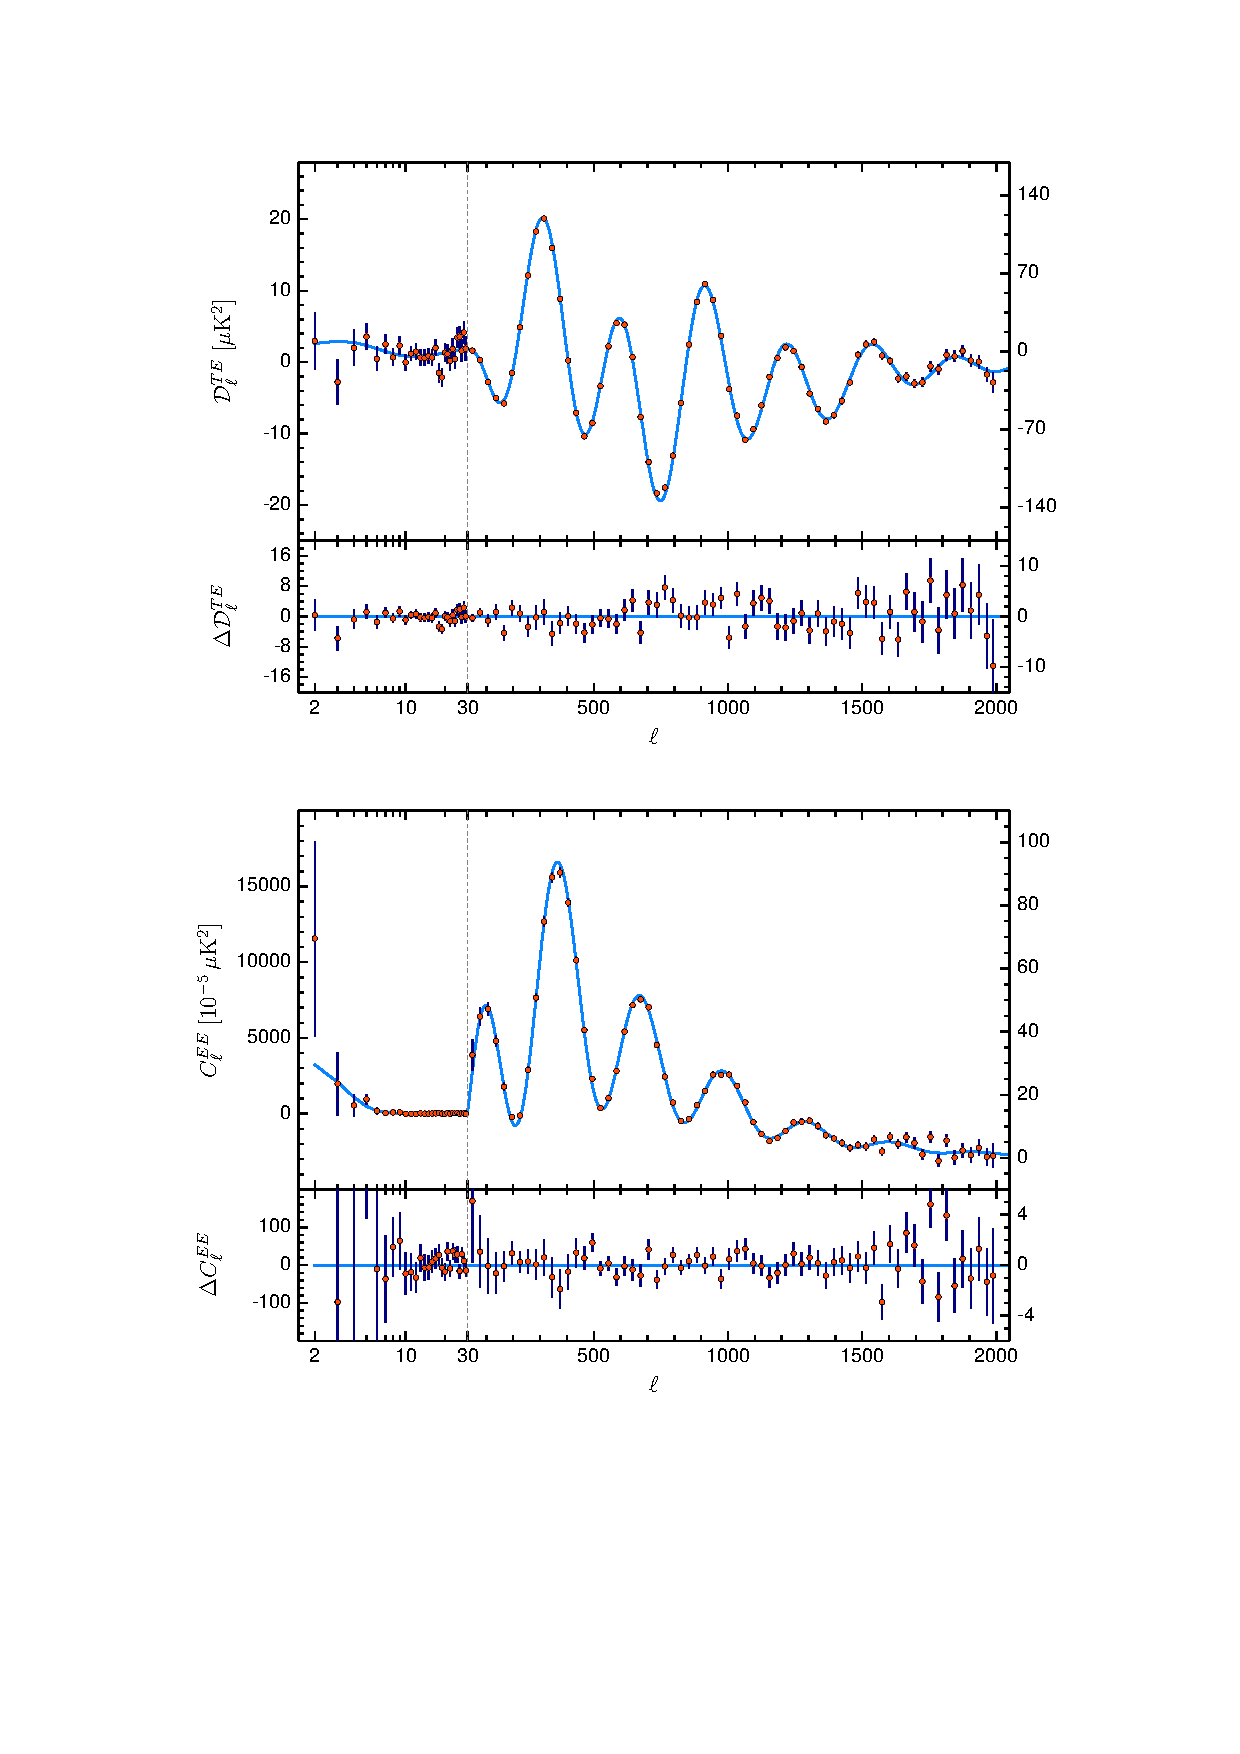
\includegraphics[width=0.9\textwidth]{plots/planck_TE_EE.pdf}
    \caption{Planck $TE$ (top) and $EE$ (bottom) power spectra~\cite{planck_collaboration_planck_2020}.}
    \label{fig:planck_te_ee}
\end{figure}
The other two power spectra are shown in figure~\ref{fig:planck_te_ee}. The main consideration with these two power spectra is to observe the way it breaks the degeneracy between $\tau_\mathrm{rei}$ and $\mathcal{A}_s$. $\tau_{\mathrm{rei}}$ suppresses the power spectrum as it suppresses the fraction of light that reaches an observer. However, the additional scattering actual causes anisotropies in the polarization power spectrum to increase. Thus, the effects of $\mathcal{A}_s$ and $\tau_\mathrm{rei}$ are similar in the $TT$ power spectrum but opposite in the $EE$ power spectrum. Thus, using all three power spectra will give the strongest constraints on the cosmological parameters.
\section{Tensions Between Weak Lensing and the CMB}
As seen, there are a total of five parameters needed to describe $\Lambda$CDM in weak lensing: $\Omega_m$, $\Omega_b$, $H_0$, $\mathcal{A}_s$, and $n_s$. This parameterization is not unique. Another common parameter, which tracks $\mathcal{A_s}$, is $\sigma_8$
\begin{equation}
	\sigma_8^2 = \left.\int\limits_0^\infty P(k,r)\left(\frac{3j_1(kr)}{kr}\right)^2\frac{k^2}{2\pi^2}dk\right|_{r=8}\,,
\end{equation}
which can be described as the amplitude of matter fluctuations at the scale $8 h^{-1}\mathrm{Mpc}$. With this parameter instead of $\mathcal{A}_s$, weak lensing gives strong constraints on $S_8 = \sigma_8\sqrt{\Omega_m/0.3}$. 

The reality is, however, that CMB measurements of some of these parameters differ between the parameters measured from weak lensing (precise results can be found in~\cite{amon_dark_2022,noauthor_planck_2018,planck_collaboration_planck_2020}). The main tension between CMB and weak lensing is the $S_8$ tension at about a $3\sigma$ difference (figure~\ref{fig:s8_tension}). The most famous discrepancy is the $H_0$ tension (figure~\ref{fig:h0_tension}). The tension is produced by a discrepancy between CMB measurements and the local cosmic distance ladder, producing a nearly $5\sigma$ difference.  There have been extensive efforts to propose a model that can resolve these tensions (early dark energy\cite{kamionkowski_hubble_2022}, quintessence~\cite{tsujikawa_quintessence_2013}, etc.), but as of now no model can simultaneously resolve both tensions. For example, early dark energy resolves the $H_0$ tension, but the $S_8$ tension tends to either remain the same or increase. The remaining chapters will explore how to compute these tensions and demonstrate a proposed consistency test.
\begin{figure}[ht]
	\centering
	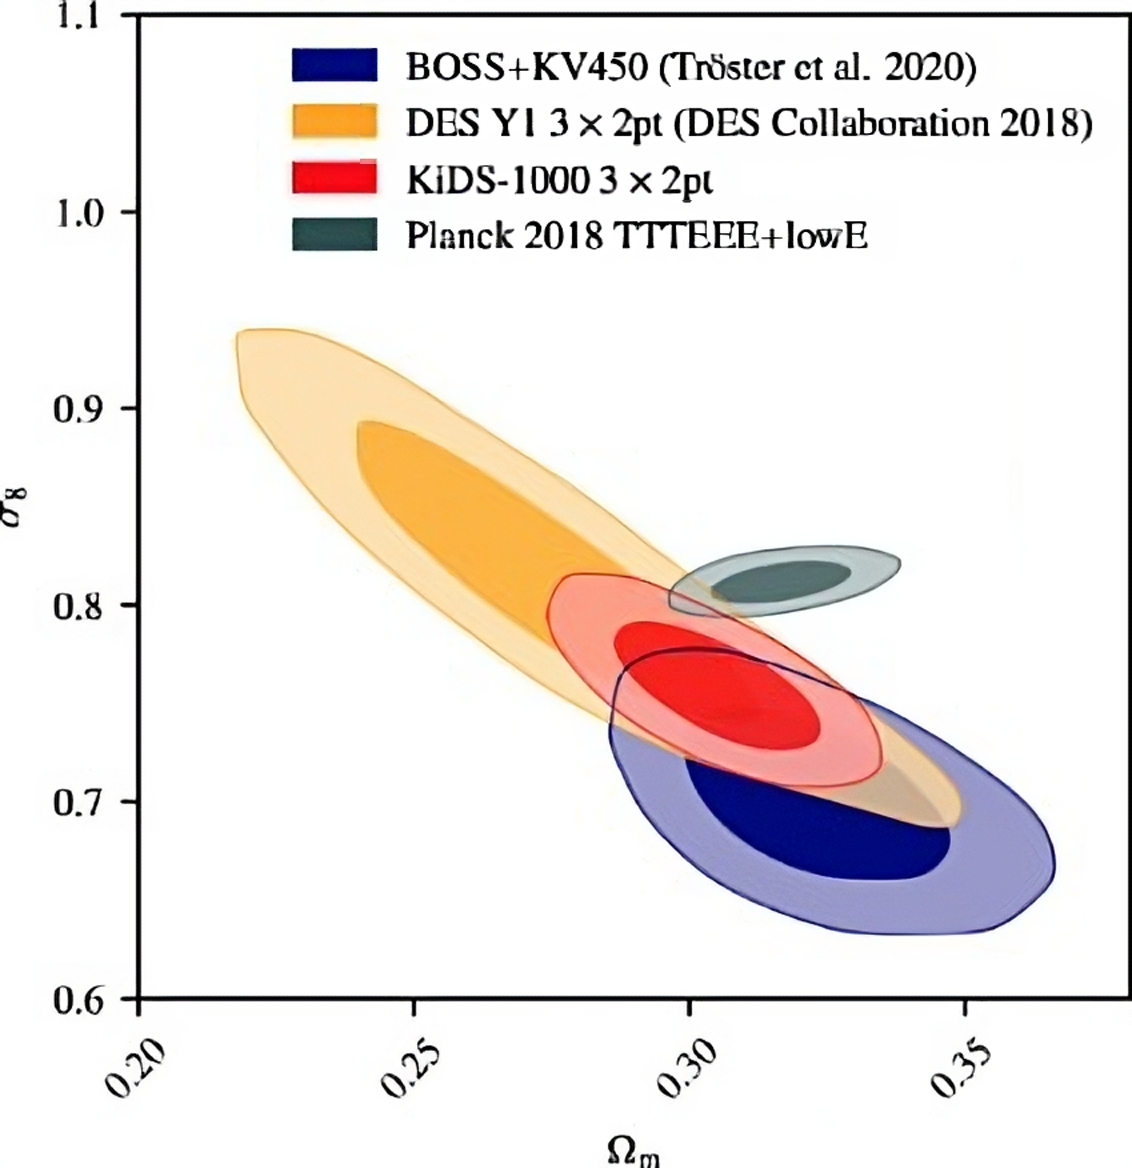
\includegraphics[width=0.75\textwidth]{plots/s8_tension_4x.jpeg}
	\caption{Measurements of $S_8$ from different experiments.}
	\label{fig:s8_tension}
\end{figure}
\begin{figure}[ht]
	\centering
	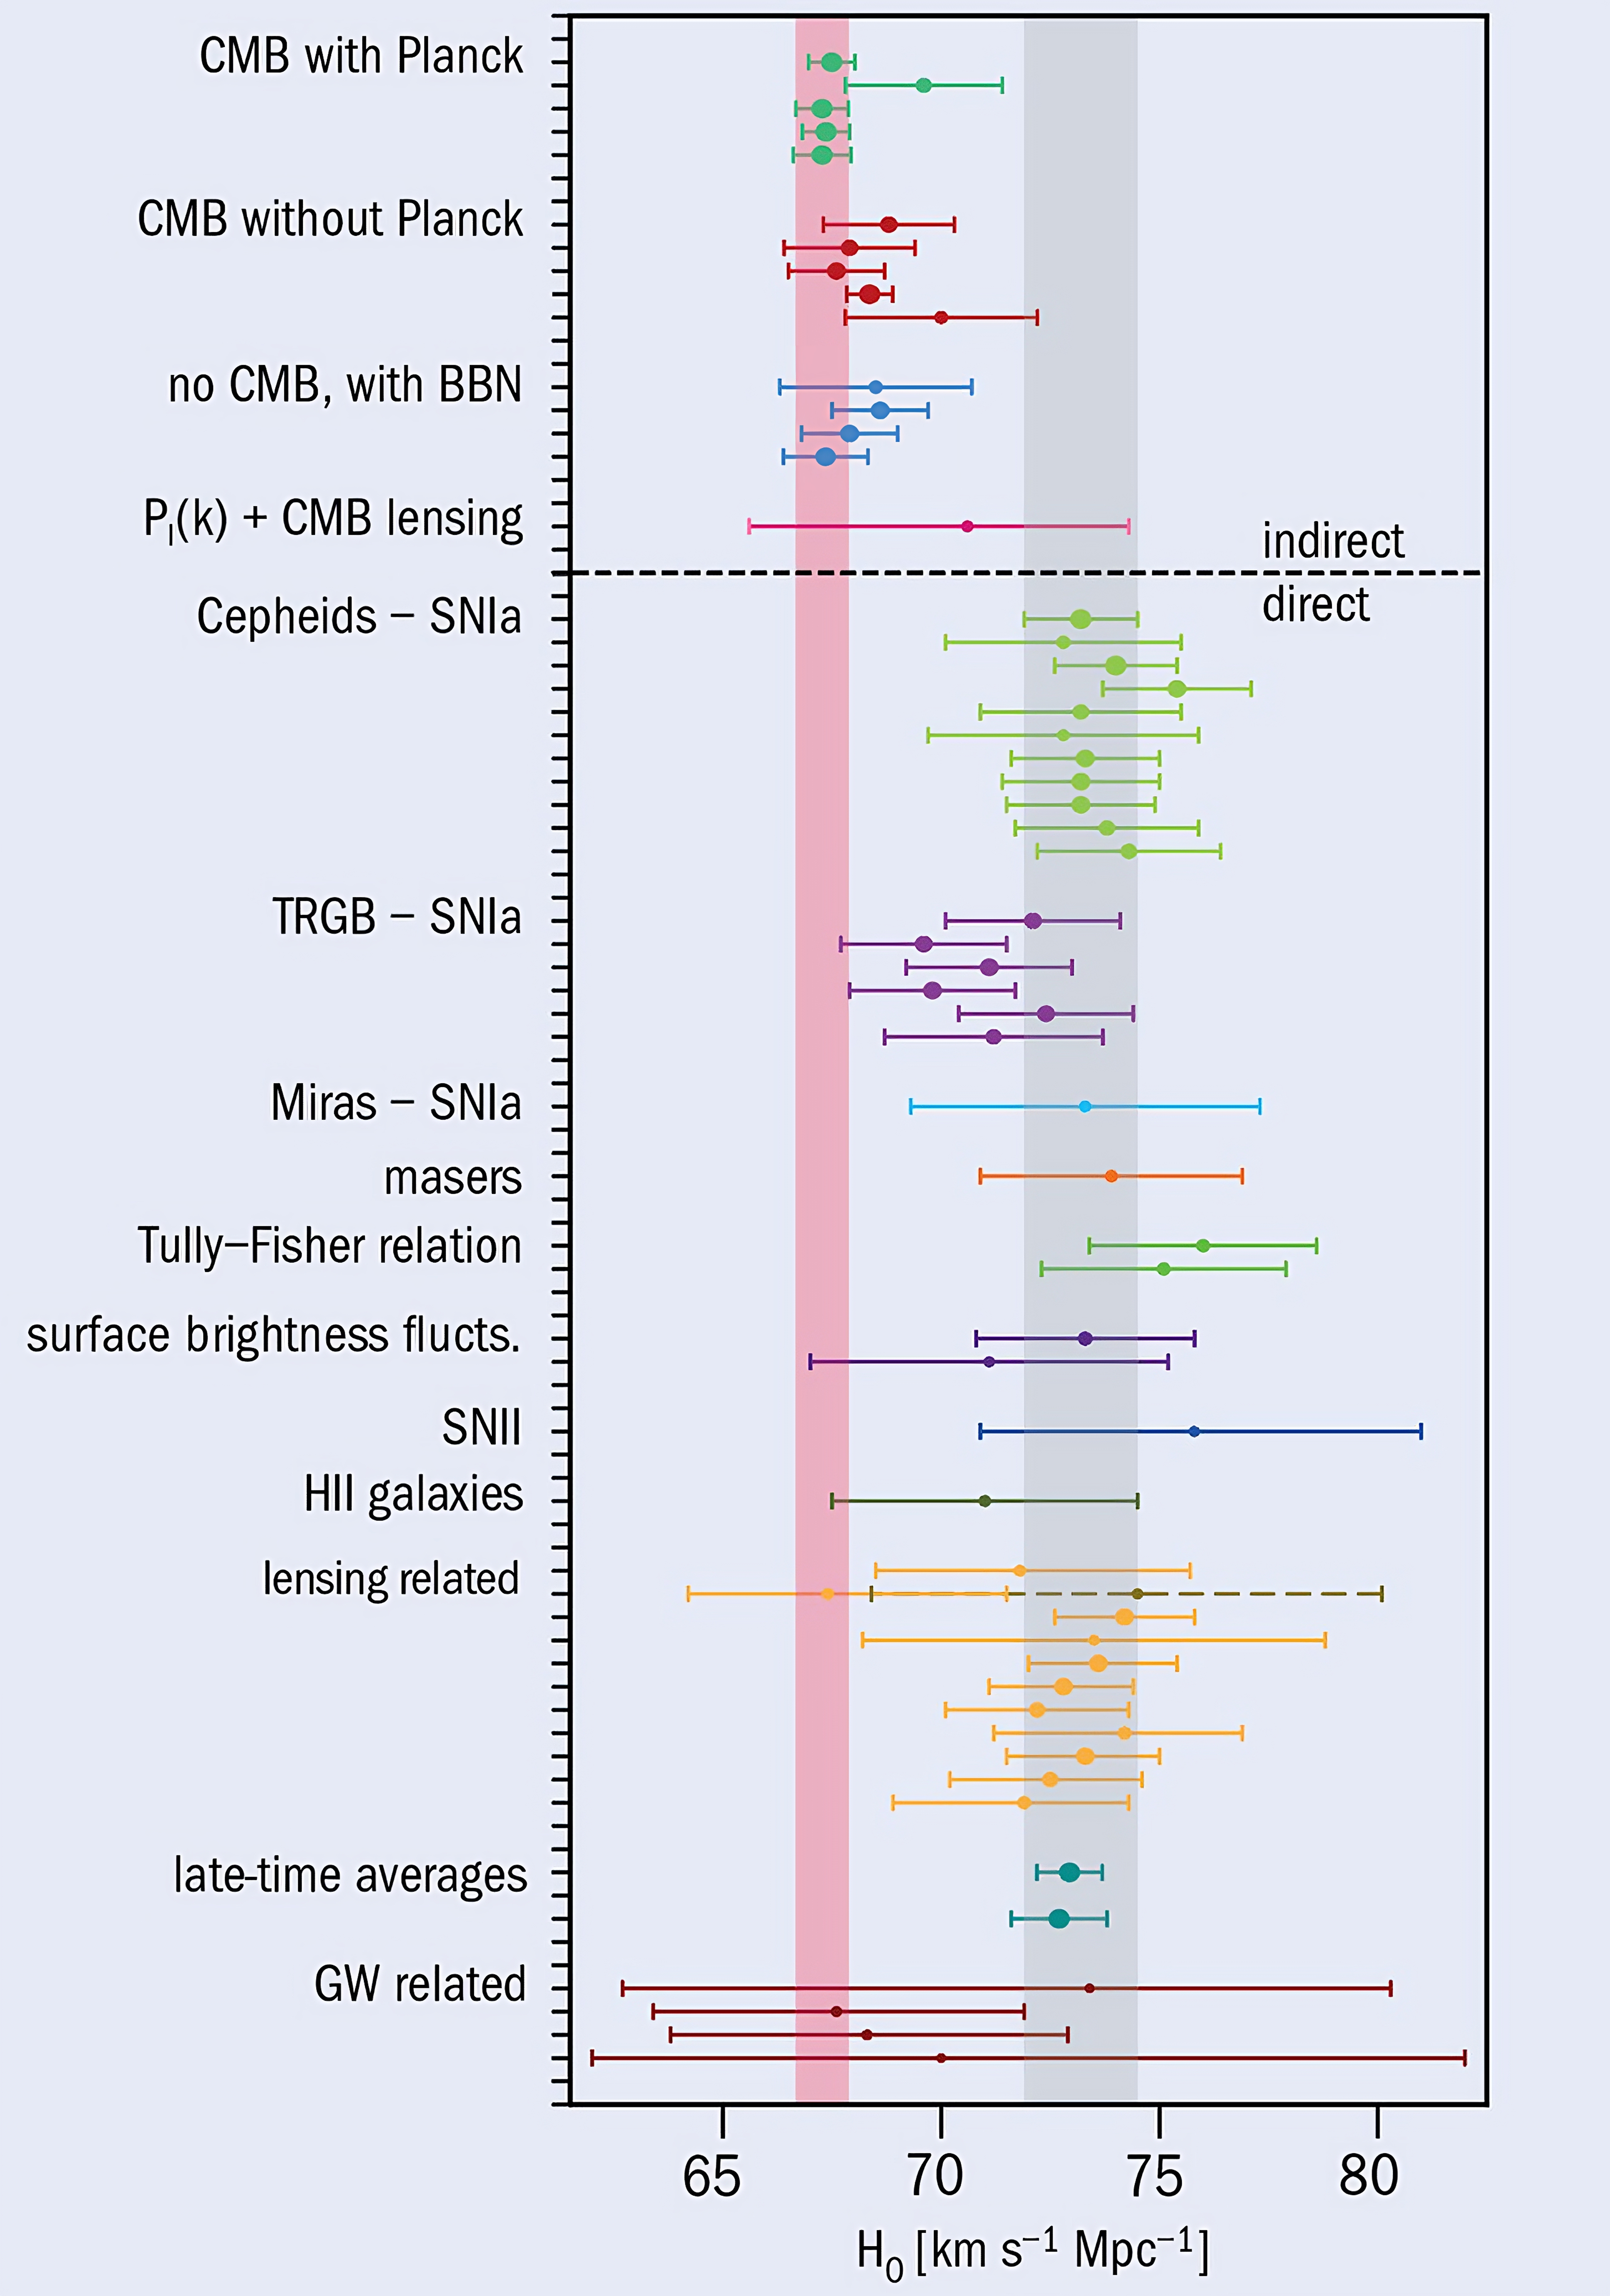
\includegraphics[width=0.75\textwidth]{plots/h0_tension_4x.jpeg}
	\caption{Measurements of $H_0$ from different experiments.}
	\label{fig:h0_tension}
\end{figure}








